\chapter{Testen}
In dit hoofdstuk wordt gekeken naar de testen die gedaan zijn tijdens het traject. Eerste, wordt gekeken naar het testplan van de hardware validatie, daarna naar het testplan voor de applicatie. Testen in softwareontwikkeling is een belangrijk onderdeel, hiermee is te zien hoe robuust de applicatie is geworden.

\section{Testplan hardware validatie} \label{sec:hwtestplan}
Dit is het testplan dat bedacht is om alle porten van de Satellite te testen. Dit is het testplan dat wordt gebruikt bij Satellite hardware. Hiermee kan Sensor Maritime heel snel de hardware verifiëren.
\subsection{DIP switch} \label{sec:dip}
De eerste drie schakelaars worden anders getest in vergelijking met de laatste vier. De laatste vier schakelaars laten vier leds branden, die op de Satellite zitten. In tabel \ref{tab:hw_val_dip_testplan} is een overzicht van het testplan te vinden:
\begin{table}[h!]
	\caption{Testplan DIP switch poorten}
	\begin{tabular}{lp{14.5cm}}
	\toprule
	\textbf{Naam} 	& \textbf{Verwachte resultaat} \\ \toprule
	PU1				& Indien aangezet, wordt de range van de analoge input 1 verhoogd naar 24 volt. Dit verhoogt de waarde wat die microcontroller leest. De waarde wordt getoond in een GUI.\\
	-				& Wordt niet getest. \\
	PU2				& Indien aangezet, wordt de range van de analoge input 2 verhoogd naar 24 volt. Dit verhoogt de waarde wat die microcontroller leest. De waarde wordt getoond in een GUI.\\
	PU3				& Indien aangezet, wordt de range van de analoge input 3 verhoogd naar 24 volt. Dit verhoogt de waarde wat die microcontroller leest. De waarde wordt getoond in een GUI. \\
	ADD0 			& Zet 3.3V op de pin van de microcontroller, als de microcontroller 3.3V detecteert wordt led 0 aangezet.\\
	ADD1 			& Zet 3.3V op de pin van de microcontroller, als de microcontroller 3.3V detecteert wordt led 1 aangezet.\\
	ADD2 			& Zet 3.3V op de pin van de microcontroller, als de microcontroller 3.3V detecteert wordt led 2 aangezet.\\
	ADD3 			& Zet 3.3V op de pin van de microcontroller, als de microcontroller 3.3V detecteert wordt led 3 aangezet.\\ \bottomrule
	\end{tabular}
	\label{tab:hw_val_dip_testplan}
\end{table}

\newpage
\subsection{Digitale output signaal} 
Alle digitale output porten voeren dezelfde actie uit. Als een LED verbonden is met de poort gaat die aan of uit gaat om de 1 seconden.
\begin{table}[h!]
	\caption{Testplan digitale output signalen}
	\begin{tabular}{lp{14.5cm}}
	\toprule
	\textbf{Naam} 	& \textbf{Verwachte resultaat} \\ \toprule
	D1	&	Als op de pin 24V staat gaat het lampje aan. Bij 0V gaat het uit. Dit gebeurt om de 1 seconden. \\
	D2	&	Als op de pin 24V staat gaat het lampje aan. Bij 0V gaat het uit. Dit gebeurt om de 1 seconden. \\
	D3	&	Als op de pin 24V staat gaat het lampje aan. Bij 0V gaat het uit. Dit gebeurt om de 1 seconden. \\
	D4	&	Als op de pin 24V staat gaat het lampje aan. Bij 0V gaat het uit. Dit gebeurt om de 1 seconden. \\ \bottomrule
	\end{tabular}
	\label{tab:hw_val_dio_testplan}
\end{table}

\subsection{Analoog input signaal}
Aan de hand van wat is beschreven in \ref{sec:dip} zal er gebruik gemaakt worden van de DIP schakelaars PU1, PU2, en PU3 om de analoge input te testen. De microcontroller heeft een 12 bit Analog to Digital Converter (ADC) \autocite{microcontroller}. Dit betekent dat het bereik van de analoge input poorten van 0 tot 4096 ($2^{12}$) is. Dus bij 24 volt zal de microcontroller ongeveer 4096 inlezen, het getal kan af en toe lager zijn in verband met ruis. Bij 0 volt zal de microcontroller 0 inlezen. PU1, PU2, PU3 zet het analoge bereik tussen 3,3 volt en 24 volt. Dit betekent als PU1, PU2 of PU3 uit staan dat het maximale bereik 3,3 volt is en als het aan staat is het bereik 24 Volt. Om het bereik te testen wordt gebruik gemaakt van een Graphical User Interface. De microcontroller zal om de 100 microseconden de analoge input omzetten naar digitale waarde en dit opsturen via UDP. Hiermee kan geverifieerd worden dat als de DIP schakelaars uitstaan het bereik van de waarden van 0 tot 1100 gaat. Als de DIP schakelaars aan staan dan zal het bereik zijn van 0 tot 4096. Hieronder is een overzicht van hoe de analoge input porten gevalideerd worden \ref{tab:hw_val_ai_testplan}.
\begin{table}[h!]
	\caption{Testplan voor de analoge input signalen}
	\begin{tabular}{lp{14.5cm}}
	\toprule
	\textbf{Naam} 	& \textbf{Verwachte resultaat} \\ \toprule
	AI1			& Als de schakelaar PU1 van de schakelaar aangezet wordt dan zal het data bereik op de graphical user interface aangepast worden naar 0 tot 4096. Als de dip schakelaar uit staat dan zal het bereik maar van 0 tot 1100 gaan.\\
	AI2			& Als de schakelaar PU1 van de schakelaar aangezet wordt dan zal het data bereik op de graphical user interface aangepast worden naar 0 tot 4096. Als de dip schakelaar uit staat dan zal het bereik maar van 0 tot 1100 gaan.\\
	AI3			& Als de schakelaar PU1 van de schakelaar aangezet wordt dan zal het data bereik op de graphical user interface aangepast worden naar 0 tot 4096. Als de dip schakelaar uit staat dan zal het bereik maar van 0 tot 1100 gaan.\\  \bottomrule
	\end{tabular}
	\label{tab:hw_val_ai_testplan}
\end{table}

\subsection{Relay}
De relay geeft bij het sluiten en het openen van de mechanische connectie een luid geluid dat op normale afstand van het apparaat te horen moet zijn. Het testplan van de relay wordt dan ook op geluid gebaseerd. De relay zal dan voor vijf seconden aangaan, en vervolgens weer voor vijf seconden uitgaan. Hieronder is een overzicht van het relay testplan \ref{tab:hw_val_relay_testplan}.

\begin{table}[h!]
	\caption{Testplan voor de relay}
	\begin{tabular}{lp{14.5cm}}
	\toprule
	\textbf{Naam} 	& \textbf{Verwachte resultaat} \\ \toprule
	Relay			& De microcontroller zet de pin van de relay voor vijf seconden hoog. Als dit gebeurt hoor je een klik te horen. Na vijf seconden zal deze pin weer laag gezet worden, dit moet ook gehoord kunnen worden.\\  \bottomrule
	\end{tabular}
	\label{tab:hw_val_relay_testplan}
\end{table}


\subsection{Seriële communicatie}
Om de seriële communicatie te testen wordt er gebruik gemaakt van een GUI. Deze GUI vraagt om gebruikers input. De gebruiker kan een tekst schrijven en deze wordt opgestuurd. De tekst heeft een limiet van 32 karakters. Er zal hier automatisch een newline karakter toegevoegd worden, zodat de microcontroller weet dat dit het einde van het gebruikersbericht is. Het bericht wordt opgestuurd naar de microcontroller en die zal de data verwerken. De microcontroller zal dan een antwoord geven. In dit antwoord vertelt de microcontroller vertellen welke variant van communicatie is gebruikt en daarna voegt het toe wat de microcontroller ontvangen heeft van de gebruiker. Hieronder is een overzicht \ref{fig:testplanserieel} hoe het testplan zal werken.

\begin{figure}[h!]
	\centering

	\label{fig:testplanserieel}
	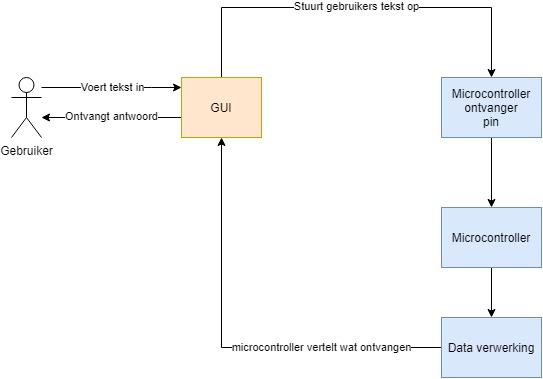
\includegraphics[width=0.5\linewidth]{voorstudie/testplan/Serieel.jpg}
	\caption{Testplan serieel communicatie}
\end{figure}

\newpage

\subsection{Graphical User Interface}
\section{Applicatie}
De applicatie moet voldoen aan de eisen en de doelstellingen die bepaald zijn in hoofdstuk \ref{ch:aanpak}. Hiervoor is gebruik gemaakt van twee manieren van testen. Ten eerste is er een GUI die data ontvangt van de Satellite en toont in de GUI in de vorm van grafieken en tabellen. Er is hiervoor een nieuw project begonnen die afstudeerder zelf ontwikkeld heeft. Voor de tweede manier van testen is door gebruik te maken van de onboard LED's die de Satellite standaard beschikt. De Satellite heeft in totaal vier LED's die de softwareontwikkelaar aan of uit kan zetten. 



\subsection{GUI}
Om de applicatie te testen is er gebruik gemaakt van een desktopapplicatie die alle data ontvangt en visualiseert in verschillende grafieken. Dit geeft de gebruiker direct input of een applicatie werkt naar behoren. Er is voor elke sensor een nieuw tabblad gemaakt. Om de applicatie goed te testen is dan ook de applicatie gebruikt op lange termijn zodat de softwareontwikkelaar ook weet of het over drie uur nog steeds zal werken. Hieronder is een voorbeeld \ref{fig:guitest} hoe de user interface eruitziet. 
\begin{figure}[h!]
	\centering
	\label{fig:guitest}
	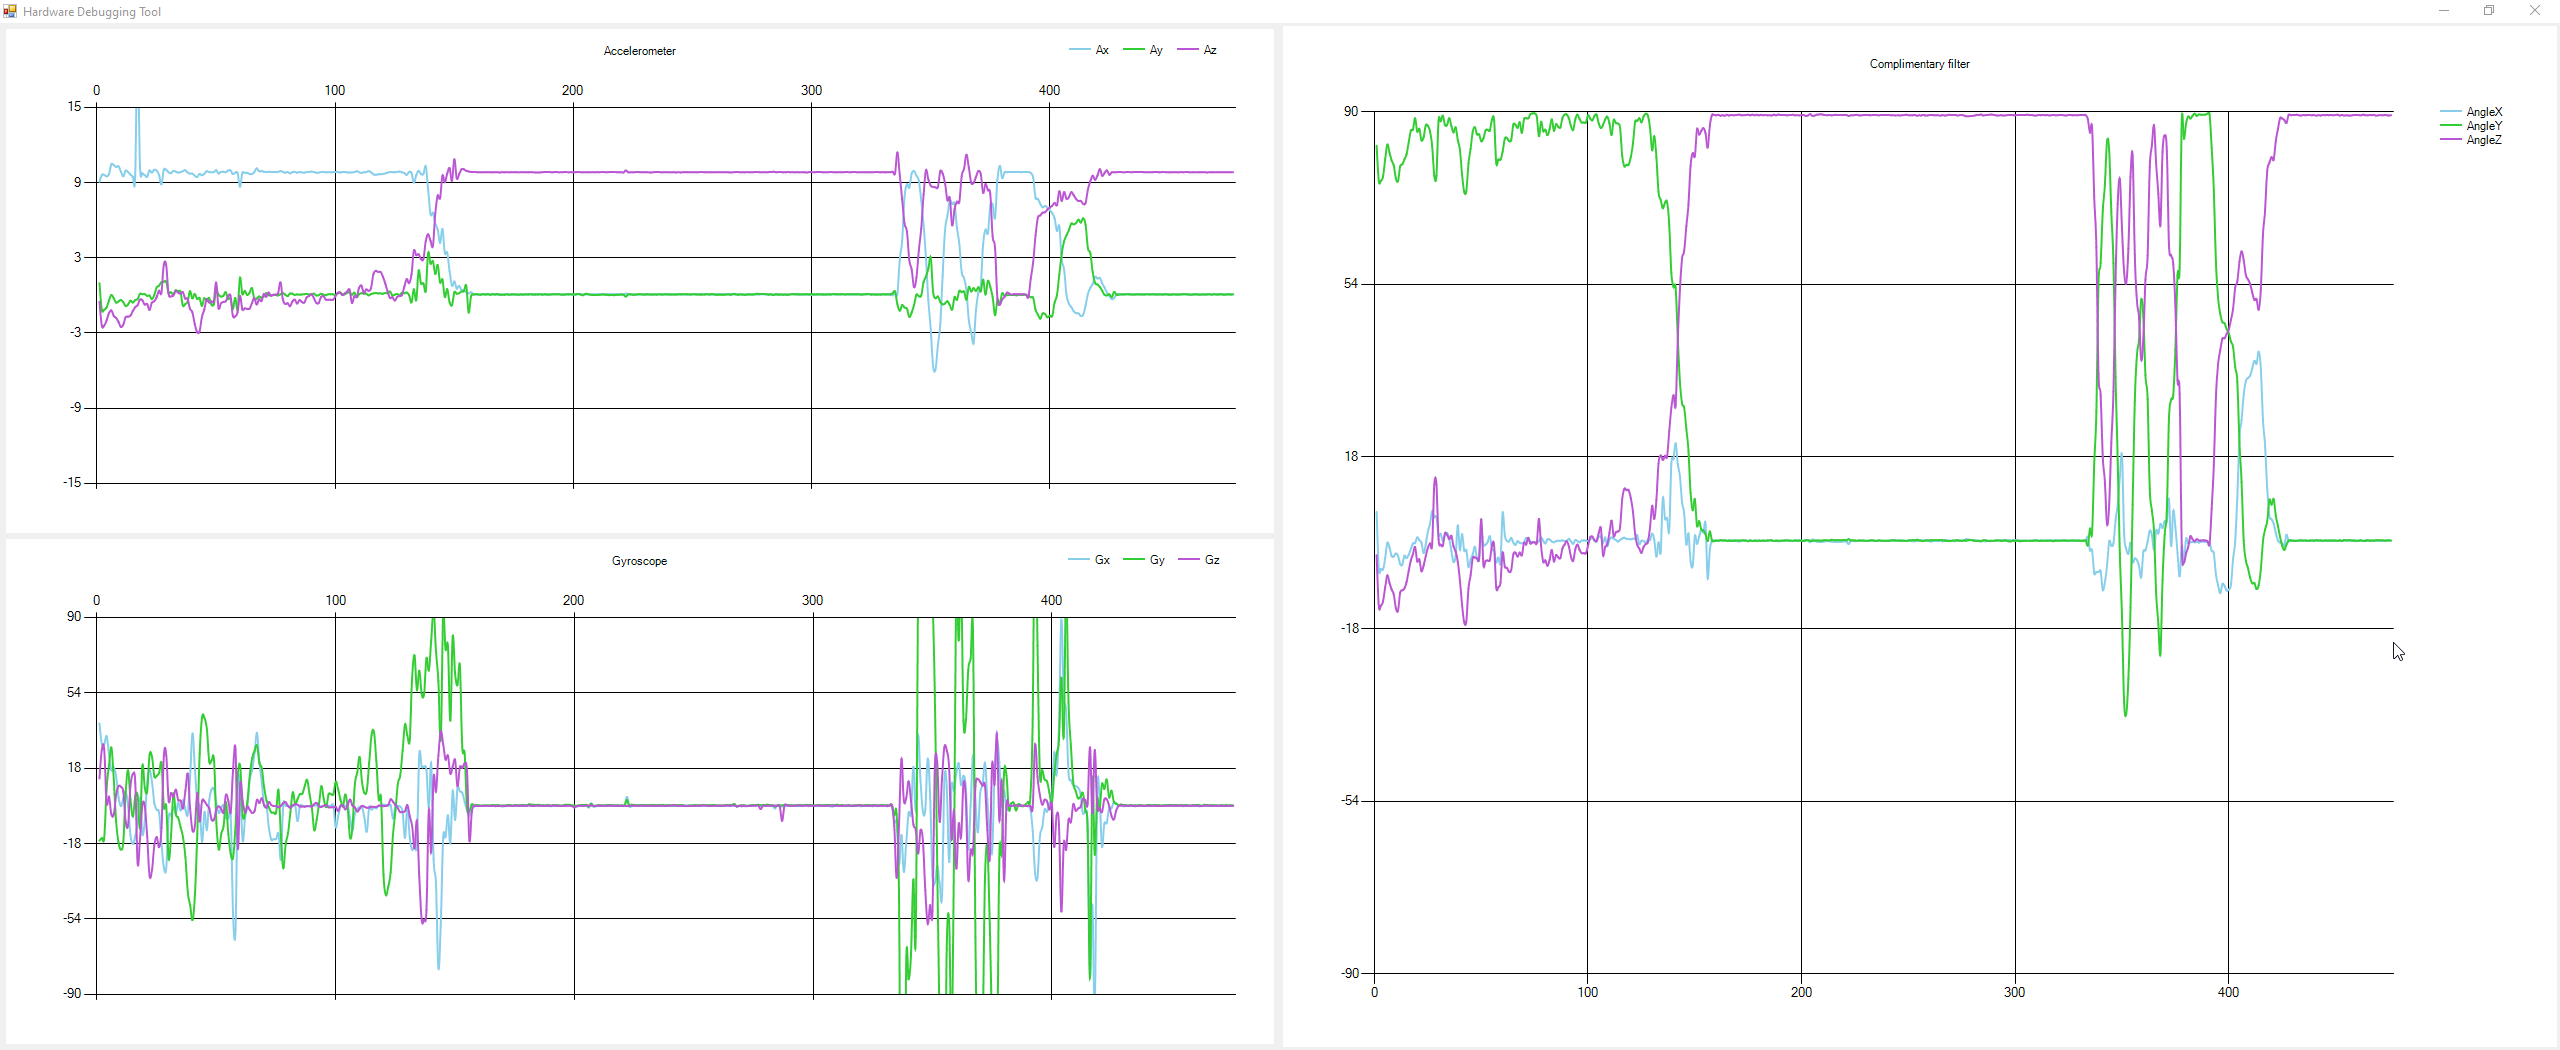
\includegraphics[width=\linewidth]{testen/GUI.png}
	\caption{Desktopapplicatie om Satellite te testen}
\end{figure}

\newpage
\subsection{LED's}
Er zitten standaard vier LED’s op het bordje, en ze hebben alle vier een andere kleur. De LED’s zijn puur voor de softwareontwikkelaar en zullen door de kapitein van een binnenvaartschip niet gezien worden. Hieronder is gedefinieerd wanneer de LED’s gebruikt worden en waarvoor ze gebruikt worden \ref{tab:leds}. Er is voor errors en warnings de standaardkleuren rood en geel gebruikt. Daarnaast wordt er voor het data ophalen een groen LED getoond als dit succesvol is gedaan, bij fouten van het ophalen van de sensor data wordt een geel of rood LED getoond. Bij het versturen van sensor data of bij het ontvangen van data wordt er een blauw licht vertoont.
\begin{table}[h!]
	\caption{Satellite onboard LED-beschrijving}
	\begin{tabular}{lp{14.5cm}}
	\toprule
	\textbf{LED Kleur} 	& \textbf{Beschrijving} \\ \toprule
	Groen	& Er wordt sensor data opgehaald\\
	Blauw	& Data wordt opgestuurd, of data is ontvangen \\
	Geel	& Er is iets fout gegaan, Satellite probeert het op te lossen\\  
	Rood	& Error \\ \bottomrule
	\end{tabular}
	\label{tab:leds}
\end{table}